% NOTE: packates que se usaran en todo el proyecto
% paquetes para el idioma
\usepackage[T1]{fontenc}
\usepackage[spanish]{babel}
\defineshorthand{"-}{\babelhyphen{hard}} % para que los guiones o dashes no se fusionen

\usepackage[utf8]{inputenc}

\usepackage[top=25mm, left=25mm, bottom=25mm, right=18mm, headheight=25mm, b5paper]{geometry}

\usepackage{graphicx} % Imagenes
\usepackage{parskip} % Arreglo de la tabulación en el documento
\usepackage{xcolor, soul} % Para poder usar colores
\usepackage{titletoc} % Para personalizar la tabla de contenido
\usepackage{titlesec} % Para personalizar los títulos de los capítulos y las secciones
\usepackage{textcomp} % Agrega el paquete textcomp en el preámbulo
\usepackage{fancyhdr} % Para trabajar con el encabezado
\usepackage{amssymb} % Agrega el paquete amssymb en el preámbulo
\usepackage{listings} % Para usar el paquete listings y sintaxis de códigos
\usepackage{lipsum} % para generar texto aleatorio
\usepackage{booktabs} % Para usar tablas personalizadas.
\usepackage{lmodern} % Latin moderno
 % packages
\graphicspath{{./assets/}}

\begin{document}

\begin{center}
	\huge\textbf{\textblue{Use useRef en React}}
	\vspace{0.5cm} % space

	
\includegraphics[width=10cm]{banner} % Logo de Lua
	\vspace{0.5cm} % space
\end{center}

En \textblue{\textbf{React}}, los Hooks son funciones especiales que permiten a los desarrolladores utilizar el estado y otras características de React sin necesidad de componentes de clase. Entre estos hooks, el Hook \lineCode{useRef} destaca como una valiosa herramienta para gestionar valores y acceder a elementos del Modelo de Objetos del Documento (Document Object Model, DOM).

El Hook \lineCode{useRef} es una herramienta poderosa que ofrece una flexibilidad y unas capacidades inmensas, pero los desarrolladores a menudo lo malinterpretan y lo utilizan incorrectamente.

En este artículo, nos adentraremos en las profundidades del Hook \lineCode{useRef}, desmitificando su propósito, funcionalidad y mejores prácticas. Al final de esta guía, comprenderás en qué consiste el Hook y obtendrás valiosos conocimientos sobre cómo aprovechar todo su potencial de forma eficaz.

\section*{¿Qué Es el Hook useRef?}

El Hook \lineCode{useRef} sirve para dos propósitos principales: almacenar valores mutables que no provocan una nueva renderización cuando se actualizan y almacenar referencias a elementos del DOM. Exploremos cómo funciona con más detalle.

Cuando un componente se renderiza en React, normalmente se restablecen su estado y otras variables. Sin embargo, hay casos en los que necesitas conservar ciertos valores incluso cuando el componente se vuelve a renderizar. Aquí es donde entra en juego el Hook \lineCode{useRef}. Te permite crear una referencia a un valor que persistirá entre renderizaciones, asegurando que el valor permanece intacto aunque cambien otras partes del componente.

Además, el Hook \lineCode{useRef} es fundamental para trabajar con elementos DOM. En React, acceder a los elementos del DOM y modificarlos directamente puede resultar complicado, especialmente sin el Hook useRef. Con useRef, puedes obtener una referencia a un elemento DOM concreto y realizar operaciones sobre él. Esto elimina la necesidad de bibliotecas externas o de complicadas soluciones.

\section*{Implementación de useRef en React}

Manipular el DOM es una tarea habitual en el desarrollo web porque te permite cambiar y actualizar dinámicamente el contenido, la estructura y la apariencia de una página web.

En el desarrollo tradicional de JavaScript, acceder y manipular elementos del DOM requería utilizar métodos como getElementById, querySelector, o getElementsByClassName para seleccionar elementos específicos del documento. Una vez seleccionados, puedes actualizar el contenido, modificar los estilos o adjuntar escuchadores de eventos.
\vspace{0.2cm} % separacion para el codigo

\begin{lstlisting}[language=TypeScript, style=mystyle]
  import { \lineCode{useRef} } from 'react';
\end{lstlisting}

Una vez importado, puedes declarar una variable ref dentro de tu componente funcional utilizando el Hook \lineCode{useRef}:
\vspace{0.2cm} % separacion para el codigo

\begin{lstlisting}[language=TypeScript, style=mystyle]
  const myRef = \lineCode{useRef}();
\end{lstlisting}

Ahora tienes un objeto ref, miRef, que puedes utilizar para almacenar valores y acceder a ellos. Para utilizar la variable myRef con cualquier elemento, asígnala a la prop ref del elemento.
\vspace{0.2cm} % separacion para el codigo

\begin{lstlisting}[language=TypeScript, style=mystyle]
  <div ref={myRef}>This is an example element</div>
\end{lstlisting}

En el ejemplo anterior, asignas al elemento div una prop ref. Esto te permite hacer referencia al elemento y acceder a él utilizando la variable myRef en cualquier otra parte del componente.

Para acceder al valor almacenado en la referencia creada, puedes utilizar la propiedad .current del objeto myRef.
\vspace{0.2cm} % separacion para el codigo

\begin{lstlisting}[language=TypeScript, style=mystyle]
  const myRefValue = myRef.current;
  console.log(myRefValue); // <div>This is a sample div</div>
\end{lstlisting}

\section*{Manipulación del DOM con el Hook useRef}

Manipular el DOM es una tarea habitual en el desarrollo web porque te permite cambiar y actualizar dinámicamente el contenido, la estructura y la apariencia de una página web.

En el desarrollo tradicional de JavaScript, acceder y manipular elementos del DOM requería utilizar métodos como \lineCode{getElementById}, \lineCode{querySelector}, o \lineCode{getElementsByClassName} para seleccionar elementos específicos del documento. Una vez seleccionados, puedes actualizar el contenido, modificar los estilos o adjuntar escuchadores de eventos.
\vspace{0.2cm} % separacion para el codigo

\begin{lstlisting}[language=HTML, style=mystyle]
  <div>
      <input type="text" id="myInput" />
      <button id="focusButton">Focus Input</button>
  </div>
   <!-- JavaScript -->
  <script>
    const inputRef = document.getElementById('myInput');
    const focusButton = document.getElementById('focusButton');
    const handleFocus = function() {
      inputRef.focus();
    };
    focusButton.addEventListener('click', handleFocus);
  </script>
\end{lstlisting}

Sin embargo, cuando se trabaja con elementos del DOM en un componente React, el proceso no es el mismo debido al DOM virtual del componente y a la necesidad de gestionar las actualizaciones de forma eficiente. A menudo, los desarrolladores recurren a diversos enfoques, como el uso de refs o librerías externas como jQuery, para acceder a los elementos del DOM y manipularlos.

Con la introducción del Hook \lineCode{useRef} en React, el proceso de trabajar con elementos DOM dentro de los componentes se ha agilizado significativamente. El Hook useRef proporciona una forma directa de crear una referencia a un elemento DOM, haciéndolo fácilmente accesible y manipulable dentro del contexto del componente.
\vspace{0.2cm} % separacion para el codigo

\begin{lstlisting}[language=TypeScript, style=mystyle]
  import { \lineCode{useRef} } from 'react';

  const FocusComponent = () => {
    const inputRef = \lineCode{useRef}(null);

    const handleFocus = () => {
      // accessing the input element
      let inputElement = inputRef.current;

     // modify the DOM element
     inputElement.focus();
    };

   return (
      <div>
        <input type="text" ref={inputRef} />
        <button onClick={handleFocus}>Focus Input</button>
      </div>
    );
  }
\end{lstlisting}

En este ejemplo, el Hook \lineCode{useRef} se utiliza para crear una referencia \lineCode{inputRef} que apunta al elemento \lineCode{input}. Cuando se pulsa el botón «Focus Input», la función \lineCode{handleFocus} utiliza\\ \lineCode{inputRef.current.focus()} para establecer directamente el enfoque en el elemento de entrada. Esto demuestra cómo el Hook useRef simplifica el proceso de trabajar con elementos DOM en React.

Otro ejemplo es que quieras manipular un \lineCode{div} cambiando su fondo cuando se pulsa un botón:
\vspace{0.2cm} % separacion para el codigo

\begin{lstlisting}[language=TypeScript, style=mystyle]
  import { \lineCode{useRef} } from 'react';

  const ExampleComponent = () => {
    const divRef = \lineCode{useRef}();

    const handleClick = () => {
      divRef.current.style.backgroundColor = 'red';
    };

    return (
      <div>
        <div ref={divRef}>This is a sample div</div>
        <button onClick={handleClick}>Change Color</button>
      </div>
    );
  }
\end{lstlisting}



En este ejemplo, creas una referencia con el Hook \lineCode{useRef} llamada \lineCode{divRef}. Asignas esta referencia a la proposición \lineCode{ref} del elemento \lineCode{div}.

Cuando se pulsa el botón «Change Color», se invoca la función handleClick. En la función, puedes acceder al elemento \lineCode{div} con \lineCode{divRef.current}. En este caso, modificas el color de fondo del elemento \lineCode{div} actualizando su propiedad \lineCode{style.backgroundColor} a «rojo».
\vspace{0.2cm} % separacion para el codigo

\begin{lstlisting}[language=TypeScript, style=mystyle]
  divRef.current.style.backgroundColor = 'red';
\end{lstlisting}

\section*{Conservar los Valores Entre Cambios de Versión}

Conservar los valores en las repeticiones es un potente caso de uso del Hook \lineCode{useRef}. Es especialmente útil cuando tienes valores que deben persistir a lo largo del ciclo de vida del componente sin provocar una nueva renderización.

Para comprender mejor este concepto, comparemos el Hook \lineCode{useRef} con el Hook \lineCode{useState} utilizando ejemplos reales:

Ejemplo con el Hook useState:
\vspace{0.2cm} % separacion para el codigo

\begin{lstlisting}[language=TypeScript, style=mystyle]
  import { useState } from 'react';

  function CounterComponent() {
    const [count, setCount] = useState(0);

    const increment = () => {
      setCount(count + 1);
    };

    return (
      <div>
        <p>Count: {count}</p>
        <button onClick={increment}>Increment</button>
      </div>
    );
  }
\end{lstlisting}

En este ejemplo, utilizas el Hook \lineCode{useState} para gestionar la variable de estado \lineCode{count}. Cada vez que se llama a la función \lineCode{increment}, el estado \lineCode{count} se actualiza utilizando setCount. Esto provoca una nueva renderización del componente, que refleja el valor \lineCode{count} actualizado.
\vspace{0.2cm} % separacion para el codigo

\begin{center}
	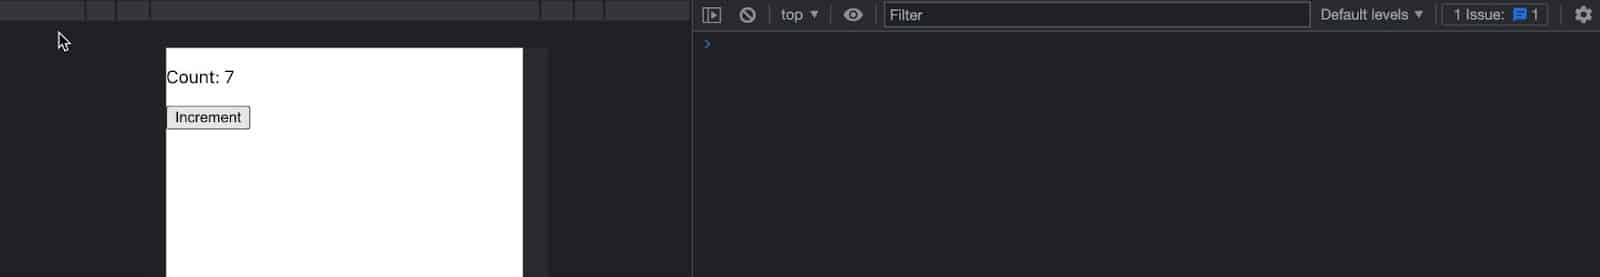
\includegraphics[width=17cm]{prueba} % Logo de Lua
\end{center}

\newpage % forzar a dar un salto de pagina

% NOTE: new page
Ejemplo con el Hook \lineCode{useRef}:
\vspace{0.2cm} % separacion para el codigo

\begin{lstlisting}[language=TypeScript, style=mystyle]
  import React, { \lineCode{useRef} } from 'react';

  function CounterComponent() {
    const countRef = \lineCode{useRef}(0);

    const increment = () => {
      countRef.current = countRef.current + 1;
      console.log('Count:', countRef.current);
    };

    return (
      <div>
        <p>Count: {countRef.current}</p>
        <button onClick={increment}>Increment</button>
      </div>
    );
  }
\end{lstlisting}

En este ejemplo, utilizas el Hook \lineCode{useRef} para crear una variable \lineCode{countRef}, inicializada con un valor inicial de \lineCode{\textbf{0}}. Cada vez que se llama a la función \lineCode{increment}, se actualiza directamente el valor \lineCode{countRef.current} sin provocar una nueva renderización. El valor actualizado se registra en la consola.
\vspace{0.2cm} % separacion para el codigo

\begin{center}
	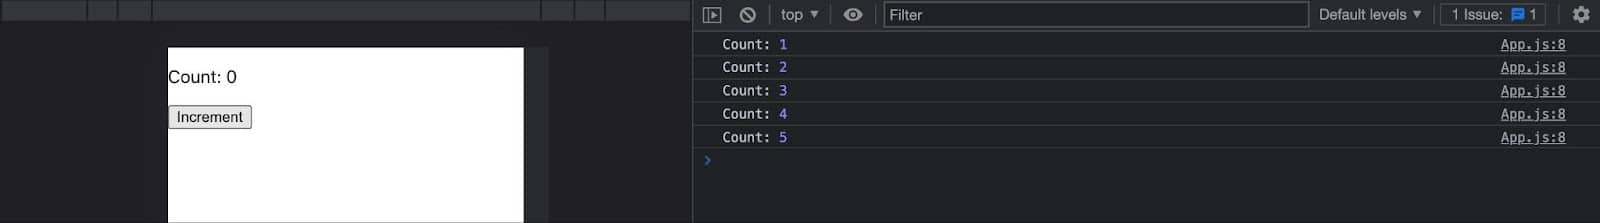
\includegraphics[width=17cm]{prueba2}
\end{center}

Al utilizar el Hook \lineCode{useRef}, el componente no se vuelve a renderizar cuando cambia el valor\\ \lineCode{countRef.current}. Esto puede ser ventajoso en situaciones en las que tengas valores que deban modificarse, pero que no afecten al proceso de renderizado.

Ten en cuenta que al utilizar el Hook \lineCode{useRef} de esta forma, los cambios en el valor \lineCode{ref} no provocarán automáticamente una nueva renderización. Si necesitas reflejar el valor actualizado en la interfaz de usuario, puedes gestionar manualmente la actualización o combinar el Hook useRef con otros hooks o variables de estado para conseguir el comportamiento deseado.

\section*{Resumen}

En este artículo, has explorado el Hook \lineCode{useRef} en React, comprendiendo su propósito, implementación y aplicaciones prácticas. Has aprendido a utilizar useRef para acceder y modificar elementos del DOM y preservar valores.

Una práctica recomendada para utilizar el Hook \lineCode{useRef} es evitar su uso excesivo. Utilízalo cuando necesites específicamente acceder y manipular elementos del DOM o preservar valores a través de re-renders.

El Hook \lineCode{useRef} también puede utilizarse para diversos escenarios prácticos, como animaciones y transiciones, almacenamiento en caché de valores o resultados intermedios, y mucho más, lo que hace que tu aplicación React destaque.

\end{document}
